\documentclass{article}

\usepackage[T1]{fontenc}
\usepackage{polski}
\usepackage[utf8]{inputenc}

\usepackage{hyperref}
\usepackage[legalpaper, margin=1.2in]{geometry}

\usepackage{listings}
\usepackage[]{algorithm2e}

\title{AEM - Zadanie nr 2}
\author{Bartosz Sobkowiak 125342 Joanna Świda 138675}
\date{07.04.2020}

\usepackage{natbib}
\usepackage{graphicx}

\begin{document}

\maketitle
\section{Opis zadania}

    Rozważany problem to zmodyfikowana wersja problemu komiwojażera. Dany jest zbiór wierzchoł-
    ków i macierz symetrycznych odległości między nimi. Zadanie polega na implementacji lokalnego przeszukiwania.  Lokalne przeszukiwanie my by¢ zaimplementowane w wersji stromej i zachłannej z dwoma różnym rodzajami sąsiedztwa.

\section{Pseudokod}

\vspace{10mm}

\begin{algorithm}[H]
     \KwData{zbiór wierchołków, macierz odległości pomiędzy wierzchołkami}
     \KwResult{najlepsze rozwiązanie}
     
    wygeneruj losowe rozwiązanie\\
    wyznacz elementy (wierzchołki) które nie znajdują się w rozwiązaniu \\
    \While{dopóki znalezione rozwiązania są lepsze}{
        \textit{# typu wyjściowego}
        \For{dla każdej pary indeksów w zakresie 0-49 w losowej kolejności} {
            oblicz deltę po operacji opdmiany wirzechołków\\
            jeśli delta jest mniejsza od 0, wstaw do obecnego rozwiązania element z listy elementów nie znajdujących się w rozwiązaniu, wedle indeksów wyznaczonych przez parę
        }\EndFor
        \textit{# typu wejściowego}
        \For{dla każdej pary indeksów w zakresie 0-49 w losowej kolejności} {
            oblicz deltę dla zamienionych wierzochołków\\
            jeśli mniejsza od zera, to zamień wierzchołki w obecnym rozwiązaniu
        }\EndFor        
        jeśli zmienione rozwiazanie jest lepsze: wybierz je jako najlepsze\\
            }
    dodaj do listy rozwiązań\\
\caption{Greedy - vertex}
\end{algorithm}

\vspace{10mm}

\begin{algorithm}[H]
     \KwData{zbiór wierchołków, macierz odległości pomiędzy wierzchołkami}
     \KwResult{najlepsze rozwiązanie}
     
    wygeneruj losowe rozwiązanie\\
    wyznacz elementy (wierzchołki) które nie znajdują się w rozwiązaniu \\
    \While{dopóki znalezione rozwiązania są lepsze}{
        \textit{# typu wyjściowego}
        \For{dla każdej pary indeksów w zakresie 0-49 w losowej kolejności} {
            oblicz deltę po operacji opdmiany wirzechołków\\
            jeśli delta jest mniejsza od najlepszej jak dotąd znalezionej delty: przypisz nową wartość najlepszej delty, wstaw do obecnego rozwiązania element z listy elementów nie znajdujących się w rozwiązaniu, wedle indeksów wyznaczonych przez parę
        }\EndFor
        \textit{# typu wejściowego}
        \For{dla każdej pary indeksów w zakresie 0-49 w losowej kolejności} {
            oblicz deltę dla zamienionych wierzochołków\\
            jeśli delta jest mniejsza od najlepszej jak dotąd znalezionej delty: przypisz nową wartość najlepszej delty, to zamień wierzchołki w obecnym rozwiązaniu
        }\EndFor        
        jeśli zmienione rozwiazanie jest lepsze: wybierz je jako najlepsze\\
            }
    dodaj do listy rozwiązań\\
\caption{Steepest - vertex}
\end{algorithm}

\vspace{10mm}

\begin{algorithm}[H]
     \KwData{zbiór wierchołków, macierz odległości pomiędzy wierzchołkami}
     \KwResult{najlepsze rozwiązanie}
     
    wygeneruj losowe rozwiązanie\\
    \While{dopóki znalezione rozwiązania są lepsze}{
        \For{dla każdej pary indeksów w zakresie 0-49 w losowej kolejności} {
            podmień krawędzie według indeksów \\
            oblicz deltę dla zamienionych krawędzi\\
            jeśli delta jest mniejsza od zera, to podmień w obecnym rozwiązaniu
        }\EndFor        
        jeśli zmienione rozwiazanie jest lepsze: wybierz je jako najlepsze\\
            }
    dodaj do listy rozwiązań\\
\caption{Greedy - edges}
\end{algorithm}

\vspace{10mm}

\begin{algorithm}[H]
     \KwData{zbiór wierchołków, macierz odległości pomiędzy wierzchołkami}
     \KwResult{najlepsze rozwiązanie}
     
    wygeneruj losowe rozwiązanie\\
    \While{dopóki znalezione rozwiązania są lepsze}{
        \For{dla każdej pary indeksów w zakresie 0-49 w losowej kolejności} {
            podmień krawędzie według indeksów \\
            oblicz deltę dla zamienionych krawędzi\\
            jeśli delta jest mniejsza od najlepszej jak dotąd znalezionej delty: przypisz nową wartość najlepszej delty, to podmień w obecnym rozwiązaniu
        }\EndFor        
        jeśli zmienione rozwiazanie jest lepsze: wybierz je jako najlepsze\\
            }
    dodaj do listy rozwiązań\\
\caption{Steepest - edges}
\end{algorithm}

\vspace{10mm}


\section{Wyniki obliczeń i wizualizacje}

\begin{table}[h!]
\centering
\begin{tabular}{ |c|c|c|c|c|c| } 
 \hline
 Zbiór & Wersja & Sąsiedztwo & Min & Avg & Max \\ 
  \hline
 kroA$_{100}$ & Greedy & Wierzchołki & 14265 & 17731 & 22737 \\ 
  \hline
 kroA$_{100}$ & Greedy & Krawędzie & 11657 & 12744 & 14762 \\ 
 \hline
 kroB$_{100}$ & Greedy & Wierzchołki & 13968 & 17413 & 22414 \\ 
 \hline
 kroB$_{100}$ & Greedy & Krawędzie & 11522 & 12705 & 14318 \\ 
 \hline
\end{tabular}
\caption{Wartości rozwiązań dla algorytmu Greedy}
\end{table}

\begin{table}[h!]
\centering
\begin{tabular}{ |c|c|c|c|c|c| } 
 \hline
 Zbiór & Wersja & Sąsiedztwo & Min & Avg & Max \\ 
 \hline
 kroA$_{100}$ & Steepest & Wierzchołki & 0.1613 & 0.3202 & 0.4985 \\ 
  \hline
 kroA$_{100}$ & Steepest & Krawędzie & 0.0924  & 0.1441 &  0.2291 \\ 
 \hline
 kroB$_{100}$ & Steepest & Wierzchołki & 0.1839 & 0.3249 &  0.5958 \\ 
 \hline
 kroB$_{100}$ & Steepest & Krawędzie & 0.0753 &  0.1329 &  0.1827 \\ 
 \hline
\end{tabular}
\caption{Czasy trwania dla algorytmu Greedy}
\end{table}

\begin{table}[h!]
\centering
\begin{tabular}{ |c|c|c|c|c|c| } 
 \hline
 Zbiór & Wersja & Sąsiedztwo & Min & Avg & Max \\ 
  \hline
 kroA$_{100}$ & Steepest & Wierzchołki & 11845 & 17736 & 22527 \\ 
  \hline
 kroA$_{100}$ & Steepest & Krawędzie & 11147 & 12676 & 15291 \\ 
 \hline
 kroB$_{100}$ & Steepest & Wierzchołki & 15084 & 17793 & 21609 \\ 
 \hline
 kroB$_{100}$ & Steepest & Krawędzie & 11322 & 12372 & 13434 \\ 
 \hline
\end{tabular}
\caption{Wartości rozwiązań dla algorytmu Steepest}
\end{table}

\begin{table}[h!]
\centering
\begin{tabular}{ |c|c|c|c|c|c| } 
 \hline
 Zbiór & Wersja & Sąsiedztwo & Min & Avg & Max \\ 
 \hline
 kroA$_{100}$ & Steepest & Wierzchołki & 0.2281 & 0.3567 & 0.7047 \\ 
  \hline
 kroA$_{100}$ & Steepest & Krawędzie & 0.1987 & 0.3554 & 1.3037 \\ 
 \hline
 kroB$_{100}$ & Steepest & Wierzchołki & 0.2504 & 0.3887 & 0.69448 \\ 
 \hline
 kroB$_{100}$ & Steepest & Krawędzie & 0.1697 & 0.3078 & 1.1066 \\ 
 \hline
\end{tabular}
\caption{Czasy trwania dla algorytmu Steepest}
\end{table}


\begin{figure}[h!]
  \centering
  \begin{minipage}[b]{0.5\textwidth}
    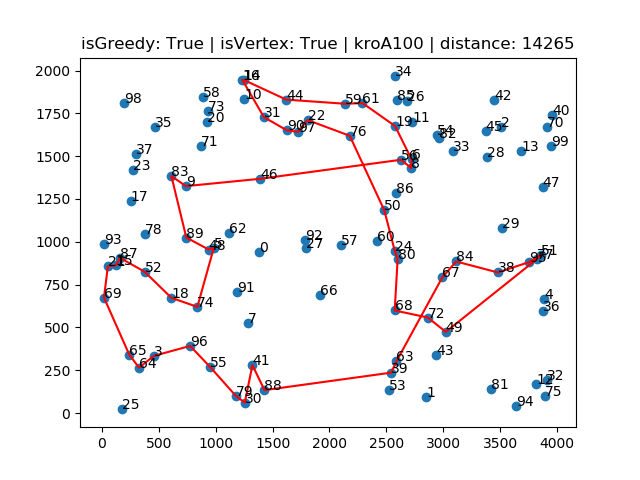
\includegraphics[width=\textwidth]{random_kroA100_V-True_G-True.png}
  \end{minipage}

  \begin{minipage}[b]{0.5\textwidth}
    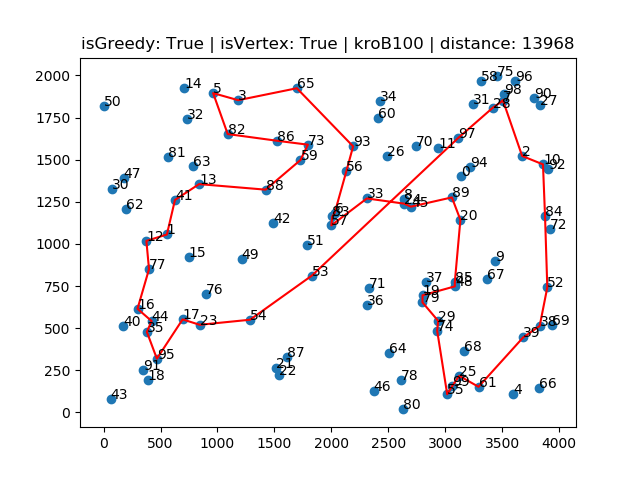
\includegraphics[width=\textwidth]{random_kroB100_V-True_G-True.png}
  \end{minipage}
  
\end{figure}
    
\begin{figure}[h!]
    \centering
  \begin{minipage}[b]{0.5\textwidth}
    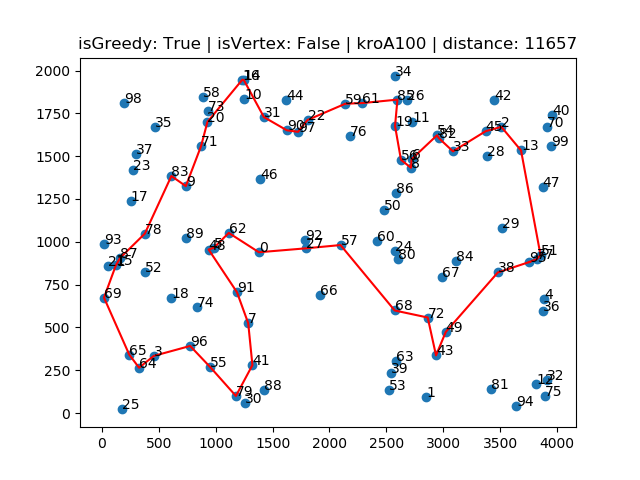
\includegraphics[width=\textwidth]{random_kroA100_V-False_G-True.png}
  \end{minipage}

  \begin{minipage}[b]{0.5\textwidth}
    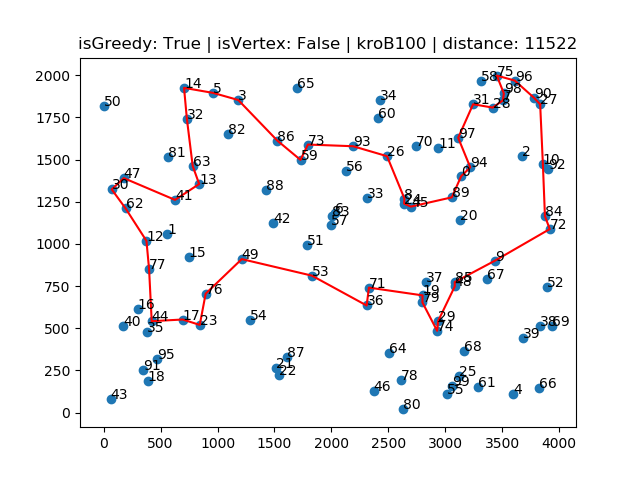
\includegraphics[width=\textwidth]{random_kroB100_V-False_G-True.png}
  \end{minipage}
\end{figure}

\begin{figure}[h!]
  \centering
  \begin{minipage}[b]{0.5\textwidth}
    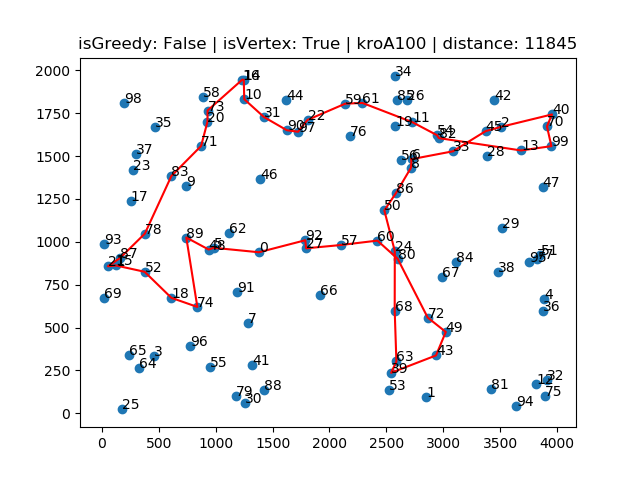
\includegraphics[width=\textwidth]{random_kroA100_V-True_G-False.png}
  \end{minipage}

  \begin{minipage}[b]{0.5\textwidth}
    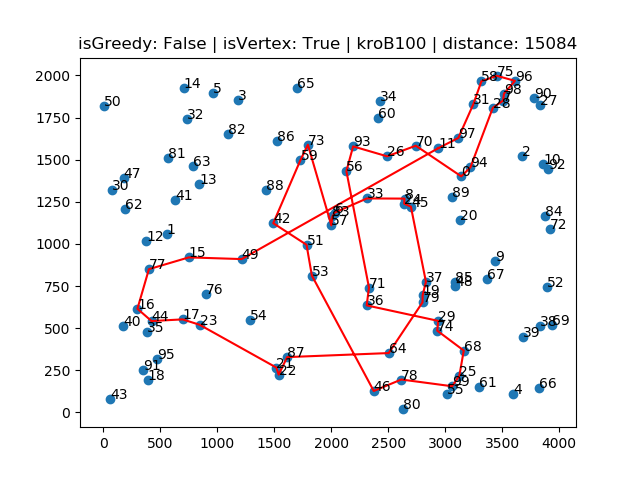
\includegraphics[width=\textwidth]{random_kroB100_V-True_G-False.png}
  \end{minipage} 
  
\end{figure}
    
\begin{figure}[h!]
    \centering
  \begin{minipage}[b]{0.5\textwidth}
    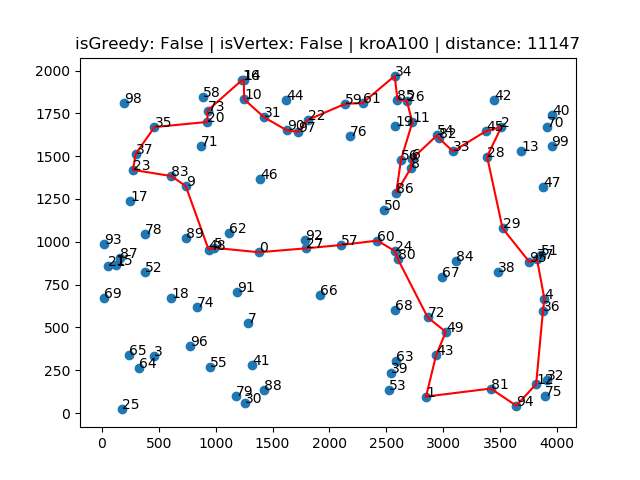
\includegraphics[width=\textwidth]{random_kroA100_V-False_G-False.png}
  \end{minipage}

  \begin{minipage}[b]{0.5\textwidth}
    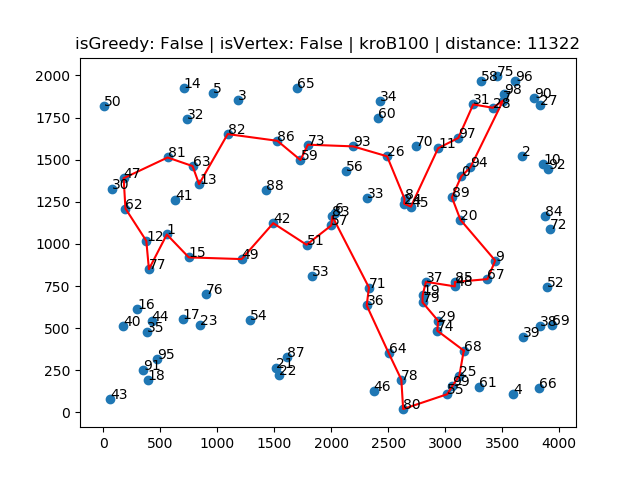
\includegraphics[width=\textwidth]{random_kroB100_V-False_G-False.png}
  \end{minipage} 
\end{figure}

\section{Wnioski}
    \subsection{Randomizacja}
    Zgodnie z zalożeniami zadania zastosowano randomizacje kolejności przeszukiwania. Indeksy krawędzi oraz indeksy punktów były generowane w kolejności pseudolosowej z wykorzystaniem pakietu numpy. W wersji zachłannej krawędzie do wstawienia i indeksy miejsca wstawienia były również generowane w losowej kolejności i zestawiane były w pary, również w kolejności losowej. Algorytm iterował po tej liście par, dzięki czemu kolejność przeglądania za każdym razem była inna.
    
    \subsection{Wnioski do problemu}
    
    Zgodnie z wiedzą poznaną podczas analizy problemu, wymiana krawędzi w problemach podobnych do problemu komiwojażera przy generowaniu losowym daje wyniki lepsze niż wymiana wierzchołków. Przy zmianie wierzchołków następuje zazwyczaj więcej przecięć trasy, co wpływa na większą długość ścieżki. Oczywiście w wersji stromej, gdy szukane jest najlepsze rozwiązanie algorytm może niekiedy dawać wyniki zbliżone do sytuacji gdy rozważana jest wymiana krawędzi. Jednak jest to obarczone dłuższym czasem obliczeń. Przy wymianie krawędzi, dla algorytmu stromego i zachłannego wyniki można uznać za porównywalne. Dla wymiany wierzchołków algorytm stromy radzi sobie w ogólności nieco lepiej.  Większy czas trwania obliczeń dla wersji stromej wynika z tego, że przeszukiwanie trwa znacznie dłużej, gdyż algorytm musi przeszukać więcej rozwiązań by znaleźć to najlepsze.
    
\section{Kod programu}

    Repozytorium z kodem algorytmów dostępne jest pod: \url{https://github.com/bbbrtk/aem}


\end{document}
